\documentclass[aspectratio=43]{beamer}

% Text packages to stop warnings
\usepackage{lmodern}
\usepackage{textcomp}
\usepackage{ulem}
\usepackage[utf8]{inputenc}
\usepackage[T1]{fontenc}

\usepackage{listings}
\usepackage{tikz}
\usetikzlibrary{arrows,decorations.pathreplacing,positioning}

% Themes
\usetheme{Boadilla}
\setbeamertemplate{footline}[page number]{}
\setbeamertemplate{navigation symbols}{}

% Suppress the navigation bar
\beamertemplatenavigationsymbolsempty

\newenvironment{changemargin}[1]{% 
  \begin{list}{}{% 
    \setlength{\topsep}{0pt}% 
    \setlength{\leftmargin}{#1}% 
    \setlength{\rightmargin}{1em}
    \setlength{\listparindent}{\parindent}% 
    \setlength{\itemindent}{\parindent}% 
    \setlength{\parsep}{\parskip}% 
  }% 
  \item[]}{\end{list}} 

\lstset{basicstyle=\scriptsize, frame=single}

\title{Lecture 21---C++11 memory model; Fine-Grained~Locking; Cache Coherency}
\subtitle{ECE 459: Programming for Performance}
\date{February 27, 2015}

\begin{document}
%%%%%%%%%%%%%%%%%%%%%%%%%%%%%%%%%%%%%%%%%%%%%%%%%%%%%%%%%%%%%%%%%%%%%%%%%%%%%%%%
\begin{frame}[plain]
  \titlepage
\end{frame}

\begin{frame}
  \frametitle{Last Time}
\begin{changemargin}{2cm}
 $\Rightarrow$ Memory ordering:
      \begin{itemize}
        \item Sequential consistency;
        \item Relaxed consistency;
        \item Weak consistency.
      \end{itemize}~\\

 $\Rightarrow$ How to prevent memory reordering with fences.\\[1em]

 Other atomic operations.

\end{changemargin}

\end{frame}
%%%%%%%%%%%%%%%%%%%%%%%%%%%%%%%%%%%%%%%%%%%%%%%%%%%%%%%%%%%%%%%%%%%%%%%%%%%%%%%%


%%%%%%%%%%%%%%%%%%%%%%%%%%%%%%%%%%%%%%%%%%%%%%%%%%%%%%%%%%%%%%%%%%%%%%%%%%%%%%%%
\part{C++11 Memory Model}
\frame{\partpage}

%%%%%%%%%%%%%%%%%%%%%%%%%%%%%%%%%%%%%%%%%%%%%%%%%%%%%%%%%%%%%%%%%%%%%%%%%%%%%%%%
\begin{frame}[fragile]
  \frametitle{Language Support: Before C/C++11}

%http://www.quora.com/C++-programming-language/How-are-the-threading-and-memory-models-different-in-C++-as-compared-to-C

  \begin{changemargin}{1.5cm}
    Before C/C++11: \\ \qquad no language-level definition of threads. (\textinterrobang)\\[1em]

    Not even a well-formed question to ask what this means:\\[.5em]
    \begin{tabular}{ll}
      \begin{minipage}{.2\textwidth}
        Thread 1:
        \begin{lstlisting}
  foo = 7;
  bar = 42;
        \end{lstlisting}
      \end{minipage} &
      \begin{minipage}{.4\textwidth}
        Thread 2:
        \begin{lstlisting}
  printf("%d\n", foo);
  printf("%d\n", bar);
        \end{lstlisting}
      \end{minipage}
    \end{tabular}
    ~\\[1em]
    \only<2>{pre C/C++11: no such thing as a thread!}
    
  \end{changemargin}
\end{frame}

%%%%%%%%%%%%%%%%%%%%%%%%%%%%%%%%%%%%%%%%%%%%%%%%%%%%%%%%%%%%%%%%%%%%%%%%%%%%%%%%
\begin{frame}
  \frametitle{Language Support in C++11: Defining the Question}

  \begin{changemargin}{1.5cm}

    Now\footnote{\url{http://www.quora.com/C++-programming-language/How-are-the-threading-and-memory-models-different-in-C++-as-compared-to-C}}:
    \begin{itemize}
    \item a memory model
    \item primitives: mutexes, atomics, memory barriers.
    \end{itemize}

    Previous example has undefined behaviour \\ \qquad per C++11. (why?)
  \end{changemargin}
\end{frame}
%%%%%%%%%%%%%%%%%%%%%%%%%%%%%%%%%%%%%%%%%%%%%%%%%%%%%%%%%%%%%%%%%%%%%%%%%%%%%%%%

%%%%%%%%%%%%%%%%%%%%%%%%%%%%%%%%%%%%%%%%%%%%%%%%%%%%%%%%%%%%%%%%%%%%%%%%%%%%%%%%
\begin{frame}[fragile]
  \frametitle{Language Support in C++11: Atomics}

  \begin{changemargin}{1.5cm}
    We've seen the notion of atomics. Here's the C++11 notation:

    \begin{lstlisting}
      atomic<int> foo, bar;      
    \end{lstlisting}
    
    \begin{tabular}{ll}
      \begin{minipage}{.25\textwidth}
        Thread 1:
        \begin{lstlisting}
  foo.store(7);
  bar.store(42);
        \end{lstlisting}
      \end{minipage} &
      \begin{minipage}{.45\textwidth}
        Thread 2:
        \begin{lstlisting}
  printf("%d\n", foo.load());
  printf("%d\n", bar.load());
        \end{lstlisting}
      \end{minipage}
    \end{tabular}

    What are the possible outputs? (good exam question!)
  \end{changemargin}
\end{frame}
%%%%%%%%%%%%%%%%%%%%%%%%%%%%%%%%%%%%%%%%%%%%%%%%%%%%%%%%%%%%%%%%%%%%%%%%%%%%%%%%


%%%%%%%%%%%%%%%%%%%%%%%%%%%%%%%%%%%%%%%%%%%%%%%%%%%%%%%%%%%%%%%%%%%%%%%%%%%%%%%%

\part{Good C++ Practice}
\frame{\partpage}

%%%%%%%%%%%%%%%%%%%%%%%%%%%%%%%%%%%%%%%%%%%%%%%%%%%%%%%%%%%%%%%%%%%%%%%%%%%%%%%%
\begin{frame}
  \frametitle{Prefix and Postfix}

  \begin{changemargin}{1.5cm}

  Lots of people use postfix out of habit, but prefix is better.\\[2em]

  In C, this isn't a problem. \\[1em]
  In some languages (like C++), it can be.
  \end{changemargin}
\end{frame}
%%%%%%%%%%%%%%%%%%%%%%%%%%%%%%%%%%%%%%%%%%%%%%%%%%%%%%%%%%%%%%%%%%%%%%%%%%%%%%%%

%%%%%%%%%%%%%%%%%%%%%%%%%%%%%%%%%%%%%%%%%%%%%%%%%%%%%%%%%%%%%%%%%%%%%%%%%%%%%%%%
\begin{frame}[fragile]
  \frametitle{Why? Overloading}

  \begin{changemargin}{1.5cm}

  In C++, you can overload the {\tt ++} and {\tt --} operators.

  \begin{lstlisting}
class X {
public:
  X& operator++();
  const X operator++(int);
...
};

X x;
++x; // x.operator++();
x++; // x.operator++(0);
  \end{lstlisting}
  \end{changemargin}
\end{frame}
%%%%%%%%%%%%%%%%%%%%%%%%%%%%%%%%%%%%%%%%%%%%%%%%%%%%%%%%%%%%%%%%%%%%%%%%%%%%%%%%

%%%%%%%%%%%%%%%%%%%%%%%%%%%%%%%%%%%%%%%%%%%%%%%%%%%%%%%%%%%%%%%%%%%%%%%%%%%%%%%%
\begin{frame}[fragile]
  \frametitle{Common Increment Implementations}

  \begin{changemargin}{1.5cm}

  Prefix is also known as {\bf increment and fetch}.

  \begin{lstlisting}
X& X::operator++()
{
  *this += 1;
  return *this;
}
  \end{lstlisting}
~\\[1em]

  Postfix is also known as {\bf fetch and increment}.

  \begin{lstlisting}
const X X::operator++(int)
{
  const X old = *this;
  ++(*this);
  return old;
}
  \end{lstlisting}
  \end{changemargin}
\end{frame}
%%%%%%%%%%%%%%%%%%%%%%%%%%%%%%%%%%%%%%%%%%%%%%%%%%%%%%%%%%%%%%%%%%%%%%%%%%%%%%%%

%%%%%%%%%%%%%%%%%%%%%%%%%%%%%%%%%%%%%%%%%%%%%%%%%%%%%%%%%%%%%%%%%%%%%%%%%%%%%%%%
\begin{frame}
  \frametitle{Efficiency}

  \begin{changemargin}{1cm}
  If you're the least concerned about efficiency, always use
  {\bf prefix} increments/decrements instead of defaulting to postfix.\\[1em]

  Only use {\tt postfix} when you really mean it, to be on the safe side.
  \end{changemargin}
\end{frame}
%%%%%%%%%%%%%%%%%%%%%%%%%%%%%%%%%%%%%%%%%%%%%%%%%%%%%%%%%%%%%%%%%%%%%%%%%%%%%%%%


%%%%%%%%%%%%%%%%%%%%%%%%%%%%%%%%%%%%%%%%%%%%%%%%%%%%%%%%%%%%%%%%%%%%%%%%%%%%%%%%
\begin{frame}
  \frametitle{Digression: The Wayside}

  \begin{center}
    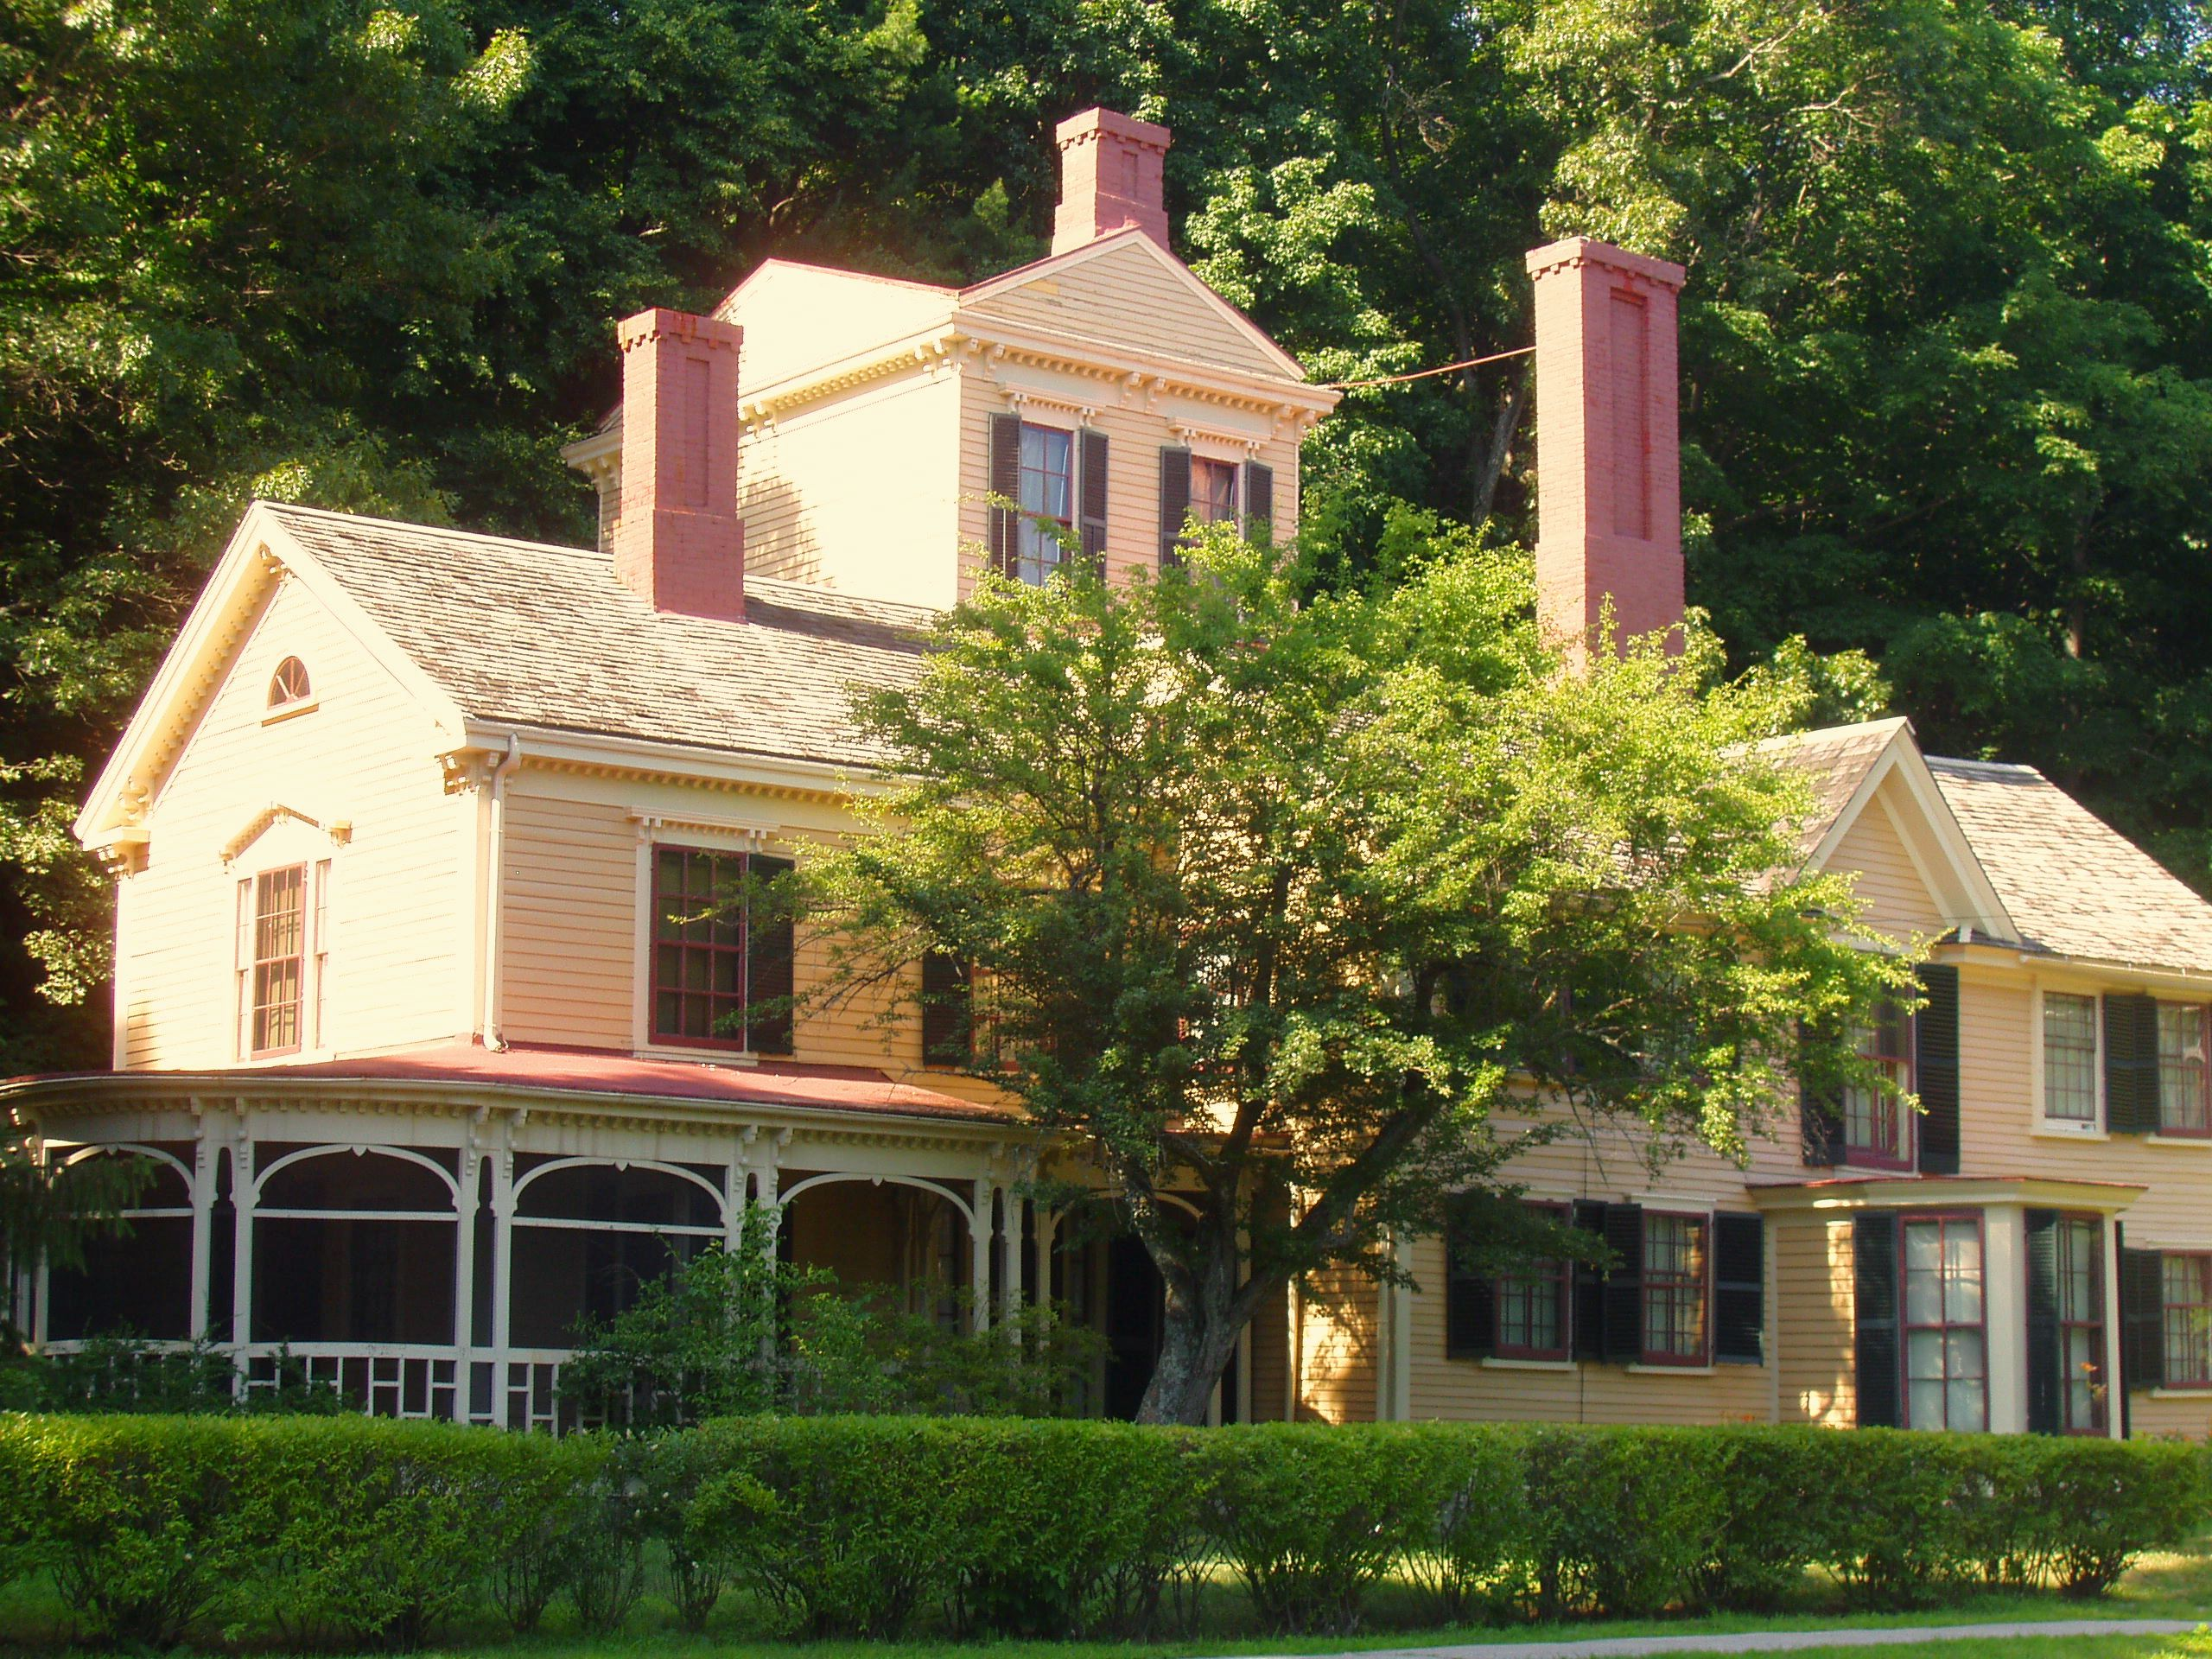
\includegraphics[width=.7\textwidth]{L21/The_Wayside_Concord_Massachusetts}
% http://en.wikipedia.org/wiki/File:The_Wayside_Concord_Massachusetts.jpg
  \end{center}
\hfill (Daderot, Wikimedia Commons)

\end{frame}
%%%%%%%%%%%%%%%%%%%%%%%%%%%%%%%%%%%%%%%%%%%%%%%%%%%%%%%%%%%%%%%%%%%%%%%%%%%%%%%%

%%%%%%%%%%%%%%%%%%%%%%%%%%%%%%%%%%%%%%%%%%%%%%%%%%%%%%%%%%%%%%%%%%%%%%%%%%%%%%%%
\begin{frame}
  \frametitle{It's Not Just Software}

\begin{changemargin}{1.5cm}
Nathaniel Hawthorne wrote:
\end{changemargin}
\begin{quote}
I have been equally unsuccessful in my architectural projects; and have transformed a simple and small old farm-house into the absurdest anomaly you ever saw; but I really was not so much to blame here as the \sout{programmer} village-carpenter, who took the matter into his own hands, and produced an unimaginable sort of thing instead of what I asked for. (January 1864)
\end{quote}

\begin{changemargin}{1.5cm}
\begin{tabular}{lrr}
Original budget:& \$500 &(\$7540 inflation-adjusted)\\
Actual cost: &\$2000 &(\$30160 inflation-adjusted)
\end{tabular}
\end{changemargin}


\end{frame}
%%%%%%%%%%%%%%%%%%%%%%%%%%%%%%%%%%%%%%%%%%%%%%%%%%%%%%%%%%%%%%%%%%%%%%%%%%%%%%%%

%% Using locks also involves a trade-off between coarse-grained locking,
%% which can significantly reduce opportunities for parallelism, and
%% fine-grained locking, which requires more careful design, increases
%% locking overhead and is more prone to bugs.

\part{Locking Granularity}
\frame{\partpage}

%%%%%%%%%%%%%%%%%%%%%%%%%%%%%%%%%%%%%%%%%%%%%%%%%%%%%%%%%%%%%%%%%%%%%%%%%%%%%%%%
\begin{frame}
  \frametitle{Locking}

  \begin{changemargin}{2cm}
  Locks prevent data races.

  \begin{itemize}
    \item Locks' extents constitute their {\bf granularity}---do you lock large sections of your program with a big lock, or do you divide the locks and protect smaller sections?
  \end{itemize}

  Concerns when using locks:

  \begin{itemize}
    \item overhead;
    \item contention; and
    \item deadlocks.
  \end{itemize}
  \end{changemargin}
\end{frame}
%%%%%%%%%%%%%%%%%%%%%%%%%%%%%%%%%%%%%%%%%%%%%%%%%%%%%%%%%%%%%%%%%%%%%%%%%%%%%%%%

%%%%%%%%%%%%%%%%%%%%%%%%%%%%%%%%%%%%%%%%%%%%%%%%%%%%%%%%%%%%%%%%%%%%%%%%%%%%%%%%
\begin{frame}
  \frametitle{Locking: Overhead}

  \begin{changemargin}{1cm}

  Using a lock isn't free. You pay:
  \begin{itemize}
    \item allocated memory for the locks;
    \item initialization and destruction time; and
    \item acquisition and release time.
  \end{itemize}

  These costs scale with the number of locks that you have.
  \end{changemargin}
\end{frame}
%%%%%%%%%%%%%%%%%%%%%%%%%%%%%%%%%%%%%%%%%%%%%%%%%%%%%%%%%%%%%%%%%%%%%%%%%%%%%%%%

%%%%%%%%%%%%%%%%%%%%%%%%%%%%%%%%%%%%%%%%%%%%%%%%%%%%%%%%%%%%%%%%%%%%%%%%%%%%%%%%
\begin{frame}
  \frametitle{Locking: Contention}

  \begin{changemargin}{1cm}
    Most locking time is wasted waiting for the lock to become available.

    How can we fix this?
      \begin{itemize}
        \item Make the locking regions smaller (more granular);
        \item Make more locks for independent sections.
      \end{itemize}
  \end{changemargin}
\end{frame}
%%%%%%%%%%%%%%%%%%%%%%%%%%%%%%%%%%%%%%%%%%%%%%%%%%%%%%%%%%%%%%%%%%%%%%%%%%%%%%%%

%%%%%%%%%%%%%%%%%%%%%%%%%%%%%%%%%%%%%%%%%%%%%%%%%%%%%%%%%%%%%%%%%%%%%%%%%%%%%%%%
\begin{frame}
  \frametitle{Locking: Deadlocks}

  \begin{changemargin}{1cm}
  The more locks you have, the more you have to worry about deadlocks.\\[1em]

  Key condition: \\ 
\qquad waiting for a lock held by process $X$ \\while holding
a lock held by process $X'$. ($X = X'$ allowed).
  \end{changemargin}

\end{frame}
%%%%%%%%%%%%%%%%%%%%%%%%%%%%%%%%%%%%%%%%%%%%%%%%%%%%%%%%%%%%%%%%%%%%%%%%%%%%%%%%

%%%%%%%%%%%%%%%%%%%%%%%%%%%%%%%%%%%%%%%%%%%%%%%%%%%%%%%%%%%%%%%%%%%%%%%%%%%%%%%%
\begin{frame}[containsverbatim]
  \frametitle{Flashback: From Lecture 1}

  \begin{changemargin}{1cm}
     Consider two processors trying to get two {\it locks}:\\[1em]
  \begin{columns}
    \column{0.4\textwidth}
      {\bf Thread 1}

      \verb+Get Lock 1+

      \verb+Get Lock 2+

      \verb+Release Lock 2+

      \verb+Release Lock 1+
    \column{0.4\textwidth}
      {\bf Thread 2}

      \verb+Get Lock 2+

      \verb+Get Lock 1+

      \verb+Release Lock 1+

      \verb+Release Lock 2+
    \end{columns}~\\[1em]
     Processor 1 gets Lock 1, then Processor 2 gets Lock 2. Oops!
          They both wait for each other \structure{(deadlock)}.
  \end{changemargin}
\end{frame}
%%%%%%%%%%%%%%%%%%%%%%%%%%%%%%%%%%%%%%%%%%%%%%%%%%%%%%%%%%%%%%%%%%%%%%%%%%%%%%%%

%%%%%%%%%%%%%%%%%%%%%%%%%%%%%%%%%%%%%%%%%%%%%%%%%%%%%%%%%%%%%%%%%%%%%%%%%%%%%%%%
\begin{frame}
  \frametitle{Key to Preventing Deadlock}

  \begin{changemargin}{2cm}

  Always be careful if \\
your code {\bf acquires a lock while holding one}.\\[1em]

  Here's how to prevent a deadlock:
  
  \begin{itemize}
    \item Ensure consistent ordering in acquiring locks; or
    \item Use {\tt trylock}.
  \end{itemize}
  \end{changemargin}
\end{frame}
%%%%%%%%%%%%%%%%%%%%%%%%%%%%%%%%%%%%%%%%%%%%%%%%%%%%%%%%%%%%%%%%%%%%%%%%%%%%%%%%

%%%%%%%%%%%%%%%%%%%%%%%%%%%%%%%%%%%%%%%%%%%%%%%%%%%%%%%%%%%%%%%%%%%%%%%%%%%%%%%%
\begin{frame}[fragile]
  \frametitle{Preventing Deadlocks---Ensuring Consistent Ordering}

  \begin{changemargin}{1cm}
  \begin{lstlisting}
void f1() {
    lock(&l1);
    lock(&l2);
    // protected code
    unlock(&l2);
    unlock(&ll);    
}

void f2() {
    lock(&l1);
    lock(&l2);
    // protected code
    unlock(&l2);
    unlock(&ll);    
}
  \end{lstlisting}

     This code will not deadlock: you can only get {\bf l2} if you have
      {\bf l1}.
  \end{changemargin}
\end{frame}
%%%%%%%%%%%%%%%%%%%%%%%%%%%%%%%%%%%%%%%%%%%%%%%%%%%%%%%%%%%%%%%%%%%%%%%%%%%%%%%%

%%%%%%%%%%%%%%%%%%%%%%%%%%%%%%%%%%%%%%%%%%%%%%%%%%%%%%%%%%%%%%%%%%%%%%%%%%%%%%%%
\begin{frame}[fragile]
  \frametitle{Preventing Deadlocks---Using {\tt trylock}}

  \begin{changemargin}{1cm}
  Recall: Pthreads' {\tt trylock} returns 0 if it gets the lock.

  \begin{lstlisting}
void f1() {
    lock(&l1);
    while (trylock(&l2) != 0) {
        unlock(&l1);
        // wait
        lock(&l1);
    }
    // protected code
    unlock(&l2);
    unlock(&ll);    
}
  \end{lstlisting}

    This code also won't deadlock: it will give up {\bf l1} if it can't get
    {\bf l2}.\\[1em]

    (BTW: trylocks also enable measuring lock contention.)

  \end{changemargin}
\end{frame}
%%%%%%%%%%%%%%%%%%%%%%%%%%%%%%%%%%%%%%%%%%%%%%%%%%%%%%%%%%%%%%%%%%%%%%%%%%%%%%%%

%%%%%%%%%%%%%%%%%%%%%%%%%%%%%%%%%%%%%%%%%%%%%%%%%%%%%%%%%%%%%%%%%%%%%%%%%%%%%%%%
\begin{frame}
  \frametitle{Coarse-Grained Locking (1)}

  \begin{center}
    
\includegraphics[scale=0.5]{L21/lock-all-the-things}

    (with one lock)
  \end{center}
\end{frame}
%%%%%%%%%%%%%%%%%%%%%%%%%%%%%%%%%%%%%%%%%%%%%%%%%%%%%%%%%%%%%%%%%%%%%%%%%%%%%%%%

%%%%%%%%%%%%%%%%%%%%%%%%%%%%%%%%%%%%%%%%%%%%%%%%%%%%%%%%%%%%%%%%%%%%%%%%%%%%%%%%
\begin{frame}
  \frametitle{Coarse-Grained Locking (2)}

  \begin{changemargin}{1cm}
  {\bf Advantages:}
  
  \begin{itemize}
    \item Easier to implement;
    \item No chance of deadlocking;
    \item Lowest memory usage / setup time.
  \end{itemize}
  \vfill
  {\bf Disadvantages:}
  \begin{itemize}
    \item Your parallel program can quickly become sequential.
  \end{itemize}
  \end{changemargin}
\end{frame}
%%%%%%%%%%%%%%%%%%%%%%%%%%%%%%%%%%%%%%%%%%%%%%%%%%%%%%%%%%%%%%%%%%%%%%%%%%%%%%%%

%%%%%%%%%%%%%%%%%%%%%%%%%%%%%%%%%%%%%%%%%%%%%%%%%%%%%%%%%%%%%%%%%%%%%%%%%%%%%%%%
\begin{frame}
  \frametitle{Coarse-Grained Locking Example---Python GIL}

  \begin{changemargin}{1cm}
  This is the main reason (most) scripting languages have poor parallel
  performance; Python's just an example.

  \begin{itemize}
    \item Python puts a lock around the whole interpreter\\ \quad (global interpreter lock).

    \item Only performance benefit you'll see from threading is if a thread is
      waiting for IO.

    \item Any non-I/O-bound threaded program will be {\bf slower} than the sequential
      version (plus, it'll slow down your system).
  \end{itemize}
  \end{changemargin}
\end{frame}
%%%%%%%%%%%%%%%%%%%%%%%%%%%%%%%%%%%%%%%%%%%%%%%%%%%%%%%%%%%%%%%%%%%%%%%%%%%%%%%%

%%%%%%%%%%%%%%%%%%%%%%%%%%%%%%%%%%%%%%%%%%%%%%%%%%%%%%%%%%%%%%%%%%%%%%%%%%%%%%%%
\begin{frame}
  \frametitle{Fine-Grained Locking (1)}

  \begin{center}
    
\includegraphics[scale=0.5]{L21/lock-all-the-things}

    (with all different locks)
  \end{center}
\end{frame}
%%%%%%%%%%%%%%%%%%%%%%%%%%%%%%%%%%%%%%%%%%%%%%%%%%%%%%%%%%%%%%%%%%%%%%%%%%%%%%%%

%%%%%%%%%%%%%%%%%%%%%%%%%%%%%%%%%%%%%%%%%%%%%%%%%%%%%%%%%%%%%%%%%%%%%%%%%%%%%%%%
\begin{frame}
  \frametitle{Fine-Grained Locking (2)}

  \begin{changemargin}{1cm}
  {\bf Advantages:}
  
  \begin{itemize}
    \item Maximizes parallelization in your program.
  \end{itemize}
  \vfill
  {\bf Disadvantages}
  \begin{itemize}
    \item May be mostly wasted memory / setup time.
    \item Prone to deadlocks.
    \item Generally more error-prone (be sure you grab the right lock!)
  \end{itemize}
  \end{changemargin}
\end{frame}
%%%%%%%%%%%%%%%%%%%%%%%%%%%%%%%%%%%%%%%%%%%%%%%%%%%%%%%%%%%%%%%%%%%%%%%%%%%%%%%%

%%%%%%%%%%%%%%%%%%%%%%%%%%%%%%%%%%%%%%%%%%%%%%%%%%%%%%%%%%%%%%%%%%%%%%%%%%%%%%%%
\begin{frame}
  \frametitle{Fine-Grained Locking Examples}

  \begin{changemargin}{1cm}
    The Linux kernel used to have {\bf one big lock}\\ that essentially made
      the kernel sequential. 
    \begin{itemize}
      \item (worked fine for single-processor systems!)
    \end{itemize}
    Now uses finer-grained locks for performance.\\[2em]

    Databases may lock fields / records / tables.\\
    \qquad  (fine-grained $\rightarrow$ coarse-grained).\\[1em]

    Can lock individual objects.
  \end{changemargin}

\end{frame}
%%%%%%%%%%%%%%%%%%%%%%%%%%%%%%%%%%%%%%%%%%%%%%%%%%%%%%%%%%%%%%%%%%%%%%%%%%%%%%%%

%%%%%%%%%%%%%%%%%%%%%%%%%%%%%%%%%%%%%%%%%%%%%%%%%%%%%%%%%%%%%%%%%%%%%%%%%%%%%%%%
\begin{frame}
  \frametitle{Live Coding Example: Midterm Tree Access Code}

  \begin{changemargin}{1cm}
    I ran the code from last year's midterm with:
    \begin{itemize}
    \item a coarse-grained lock;
    \item per-item fine-grained locks.
    \end{itemize}
    Fine-grained locks were suspiciously fast.
    
  \end{changemargin}

\end{frame}
%%%%%%%%%%%%%%%%%%%%%%%%%%%%%%%%%%%%%%%%%%%%%%%%%%%%%%%%%%%%%%%%%%%%%%%%%%%%%%%%

\section{}
%%%%%%%%%%%%%%%%%%%%%%%%%%%%%%%%%%%%%%%%%%%%%%%%%%%%%%%%%%%%%%%%%%%%%%%%%%%%%%%%
\begin{frame}
  \frametitle{Summary}

  \begin{changemargin}{1.5cm}
 C++11 memory model.\\
 
 Good increment practice. \\

 Lock granularity.

  \end{changemargin}
\end{frame}
%%%%%%%%%%%%%%%%%%%%%%%%%%%%%%%%%%%%%%%%%%%%%%%%%%%%%%%%%%%%%%%%%%%%%%%%%%%%%%%%

\end{document}
